
\begin{center}
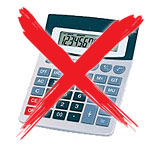
\includegraphics[scale=0.2]{no_calculator}
\end{center}

\serie{Racines et opérations}



\begin{exercice}
\begin{enumerate}
\item Ecrire les nombres ci-dessous sous la forme $a \sqrt{2}$  où $a$ désigne un nombre entier. On détaillera les étapes.\\

\begin{tabular}{m{3.8cm}m{3.5cm}}
A = $\sqrt{8}$ & B = $\sqrt{32}$\\
&\\
C = $\sqrt{200}$ & D = $2\sqrt{18}$\\
&\\

\end{tabular}

\item Ecrire les nombres ci-dessous sous la forme $a \sqrt{3}$  où $a$ désigne un nombre entier. On détaillera les étapes.

\begin{tabular}{m{3.8cm}m{3.5cm}}
E = $\sqrt{12}$ & F = $\sqrt{75}$\\
&\\
G = $5\sqrt{48}$ & H = $-10\sqrt{27}$\\
&\\

\end{tabular}

\item Ecrire les nombres ci-dessous sous la forme $a \sqrt{b}$  où $a$ et $b$ sont deux entiers avec $b$ le plus petit possible. On détaillera les étapes.

\begin{tabular}{m{3.8cm}m{3.5cm}}
I = $\sqrt{108}$ & J = $\sqrt{128}$\\
&\\
K = $3\sqrt{24}$ & L = $5\sqrt{98}$\\
&\\
M = $-3\sqrt{180}$ &\\
&\\
\end{tabular}
\end{enumerate}

\end{exercice}


\begin{exercice}

Réduire les sommes suivantes:\\

A = $\sqrt{50}+3\sqrt{2}$\\

B = $5\sqrt{3}-\sqrt{12}$\\

C = $\sqrt{20}+4\sqrt{5}-8\sqrt{45}$\\

D = $-7\sqrt{24}+2\sqrt{54}-\sqrt{150}$\\
\end{exercice}


\begin{exercice}

Réduire les sommes suivantes:\\

A = $\sqrt{8}+\sqrt{18}+\sqrt{50}$\\

B = $3\sqrt{5}+4\sqrt{125}-7\sqrt{45}$\\

C = $\sqrt{40}-2\sqrt{250}-\sqrt{160}$\\

D = $\sqrt{28}+\sqrt{63}-\sqrt{700}+\sqrt{112}$\\

\end{exercice}

\begin{exercice}
Montrer que les nombres suivants sont des entiers:\\

\begin{tabular}{m{3.8cm}m{3.5cm}}
A = $\dfrac{\sqrt{45}}{\sqrt{5}}$ & B = $\dfrac{\sqrt{128}}{\sqrt{32}}$\\
&\\
C = $\sqrt{3} \times \sqrt{12}$ & D = $\sqrt{48} \times \sqrt{\dfrac{1}{3}}$\\
&\\
E = $\dfrac{4\sqrt{7}}{\sqrt{28}}$ & F = $8\sqrt{15} \sqrt{\dfrac{3}{5}}$\\
&\\


\end{tabular}
\end{exercice}

\begin{exercice}
Sans utiliser de valeurs approchées, montrer que trois de ces nombres sont égaux:\\

\begin{tabular}{m{3.8cm}m{3.5cm}}
A = $\sqrt{5}+\sqrt{5}$ & B = $\dfrac{\sqrt{500}}{5}$\\
&\\
C = $2\sqrt{5} \sqrt{5}$ & D = $\sqrt{5+5}$\\
&\\
E = $\sqrt{20}$ &\\
&\\


\end{tabular}
\end{exercice}

\begin{exercice}

Ecrire les expressions ci-dessous sous la forme $a \sqrt{b}$  où $a$ et $b$ sont deux entiers avec $b$ le plus petit possible.\\

\begin{tabular}{m{3.8cm}m{3.5cm}}
A = $5\sqrt{6} \times 2\sqrt{3}$ & B = $\sqrt{75}+7\sqrt{3}-2\sqrt{27}$\\
&\\
C = $\sqrt{6} \times \sqrt{42}$ &\\
&\\

\end{tabular}

D = $2\sqrt{18}-3\sqrt{50}+100\sqrt{2}$ \\
\end{exercice}

\serie{Racines et dénominateurs}

\begin{exercice}
Transformer les écritures suivantes pour obtenir un dénominateur entier:\\

\begin{tabular}{m{3.8cm}m{3.5cm}}
A = $\dfrac{5}{\sqrt{7}}$ & B = $-\dfrac{8}{\sqrt{13}}$\\
&\\
C = $\dfrac{3}{\sqrt{6}}$ & D = $\dfrac{4}{3\sqrt{3}}$\\
&\\
E = $\dfrac{2-\sqrt{2}}{\sqrt{2}}$ &\\
&\\


\end{tabular}
\end{exercice}

\begin{exercice}
Transformer les écritures suivantes pour obtenir un dénominateur entier:\\

\begin{tabular}{m{3.8cm}m{3.5cm}}
A = $\dfrac{3}{\sqrt{2}+1}$ & B = $\dfrac{7}{\sqrt{3}-2}$\\
&\\
C = -$\dfrac{\sqrt{7}}{6+\sqrt{7}}$ & D = $\dfrac{\sqrt{5}+1}{\sqrt{5}-1}$\\
&\\
E = $\dfrac{3-\sqrt{11}}{4+\sqrt{11}}$ &\\
&\\

\end{tabular}

\end{exercice}

%%%%%%%%%%%%%%%%%%%%%%%%%%%%%%%%%%%%%%%%%%%%%%%%%%%

\serie{Divers}

\begin{exercice}
On considère un carré de côté $\sqrt{3} + 3$ cm 

et un rectangle dont les  dimensions  sont:

 $\sqrt{72}+ 3\sqrt{6}$ cm  et $\sqrt{2}$ cm .

Démontrer que ce carré et ce rectangle ont la même aire.
\end{exercice}


\begin{exercice}
Le tableau ci-dessous est-il un tableau de proportionnalité?

Justifier votre réponse.
%\begin{center}
%\includegraphics[scale=0.5]{R2}
%\end{center}
\end{exercice} 


\begin{exercice}
Soit P le nombre défini par : P = $\left( 2 \sqrt{5}+\sqrt{8}\right) ^2$.

\begin{enumerate}
\item Ecrire P sous la forme $a+b\sqrt{c}$ où $a$, $b$ et $c$ sont des entiers, $c$ le plus petit possible.
\item Quel nombre positif a pour carré $59+30\sqrt{2}$?
\end{enumerate}
\end{exercice} 

\begin{exercice}

\begin{enumerate}
\item Démontrer que $\sqrt{48}+\sqrt{108}=\sqrt{300}$.
\item Démontrer que $4\sqrt{18} \times \sqrt{24}=48\sqrt{3}$.
\end{enumerate}
\end{exercice} 

\begin{exercice}
On considère les nombres suivants:

A = $2\sqrt{27}-2\sqrt{3}+\sqrt{12}$ et 

B = $\sqrt{75}+\sqrt{48}-7\sqrt{3}$.

Montrer en détaillant les calculs que $\dfrac{\text{A}}{\text{B}}$ est un nombre entier.
\end{exercice} 








